% !TEX encoding = UTF-8
% !TEX TS-program = pdflatex
% !TEX root = ../Lahmer_Abdelilah_tesi.tex
% !TEX spellcheck = it-IT

%**************************************************************
\chapter{Il Progetto}
\label{cap:progetto}
%**************************************************************

%\intro{Brevissima introduzione al capitolo}\\

%**************************************************************
\section{Interesse aziendale nello stage}

Sopra Steria Group S.p.A. è un'azienda ben strutturata e affermata in molti settori, nonostante conti diversi anni alle sue spalle è in costante espansione e rinnovazione. \\

Il suo ruolo svolto in Italia non fa eccezione, per questo l'area personale è sempre in cerca di nuove risorse da inserire nelle diverse Business Unit. Non mi ha stupito quindi il fatto che abbia attivato una convenzione con l'Università di Padova e partecipi agli eventi STAGE-IT per accogliere iniziative di stage sia curricolare che retribuito.\\

La politica aziendale prevede una decorrenza di sei mesi per completare il ciclo di stage. Successivamente, nella maggioranza dei casi, vi è la propensione all'assunzione, in quanto la nuova risorsa è considerata pronta per essere effettivamente inserita nei team di sviluppo.\\

Il tirocinio è quindi visto dall'azienda come uno strumento utile a contribuire alla selezione di nuovi talenti e verificare che da entrambe le parti vi sia un interesse a proseguire il rapporto lavorativo.
\newpage
%**************************************************************
\section{Il progetto all'interno dell'azienda}

Il corso di studi rende obbligatorio lo svolgimento di uno stage che deve ricoprire un ammontare di 300-320 ore totali. È stato dunque stabilito che il lavoro di stage doveva svolgersi in 320 ore nell'arco di 8 settimane: i tempi di consegna delle funzionalità relative al progetto richiesti dall'azienda superavano la data prevista di fine stage, ciò ha permesso che lo svolgimento del progetto non subisse ulteriori vincoli temporali.\\
	
Il progetto di stage consiste nello studio delle tecnologie necessarie alla programmazione web in ambito Java EE e l'implementazione di funzionalità aggiuntive per un applicativo web per la gestione di finanziamenti in ambiente bancario. Esso è funzionante da anni presso il cliente e continuamente oggetto di evoluzioni. Tale prodotto segue l'architettura Java EE ed il suo sviluppo è vincolato alla compatibilità richiesta dal cliente per i suoi operatori di sportello, che effettivamente lo utilizzano in ambiente di produzione.\\
	
Dopo una prima fase di formazione sulle tecnologie ed una di esercitazione secondo i metodi aziendali di sviluppo, quindi, il lavoro di stage si è concentrato su questo software, chiamato ELISE. Ho portato avanti il suo ampliamento aggiungendo le nuove funzionalità il cui sviluppo mi è stato assegnato.
	
	\begin{figure}[H]
		\centering
	   	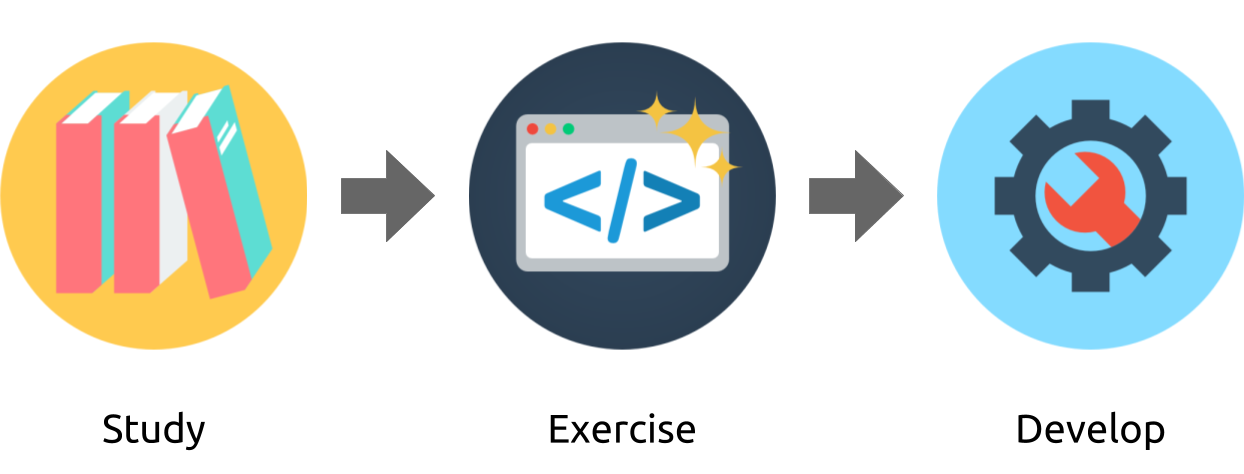
\includegraphics[width=1\textwidth]{immagini/fasi_progetto}
	   	\caption{Le fasi principali del progetto di stage}
	\end{figure}

	\subsection{ELISE}
	
	ELISE (Extended Loans Integrated System) è un sistema per la gestione integrata di tutte le problematiche di business relative all'area dei finanziamenti. È in sviluppo per il Banco Popolare, il più grande gruppo bancario in Italia a matrice cooperativa, nato ufficialmente il 1º luglio 2007 dalla fusione fra il Banco Popolare di Verona e Novara e la Banca Popolare Italiana.\\
	
	ELISE si basa su un accesso ad utenza a cui sono predisposte delle abilitazioni. Ogni utente appartiene ad una filiale operativa e risulta responsabile di determinate attività da svolgere mediante l'applicazione: richiesta di attivazione finanziamenti, verifica della documentazione, gestione pratiche di accollo o surroga, ecc. Normalmente gli utenti hanno solo determinate funzioni abilitate per sicurezza, la sede centrale invece possiede tutti i privilegi di operatività.\\
	
	I sistemi informativi di produzione in cui risiede l'applicazione web, sono in gestione presso una società ICT\glossario\ di terze parti. Tramite i loro server, il software è configurato alla comunicazione con un altro ambiente, quello di gestione dei dati, implementato su mainframe CICS\glossario\ basato appunto sulle transazioni dati.
	
	\begin{figure}[H]
		\centering
	   	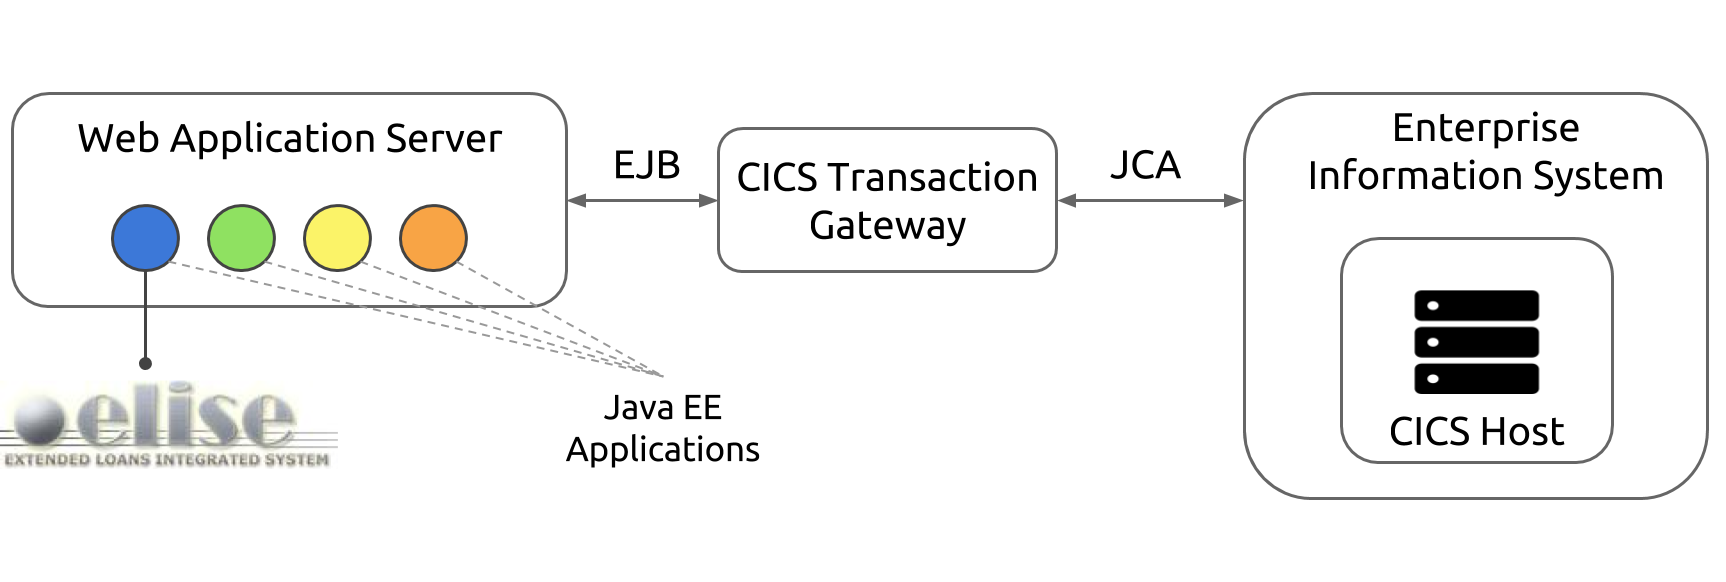
\includegraphics[width=1\textwidth]{immagini/architettura_ELISE}
	   	\caption{Architettura dei sistemi di comunicazione tra ELISE e l'ambiente CICS, implementata mediante Enterprise JavaBeans\glossario\ e le tecnologie CTG\glossario\ e JCA\glossario\ }
	\end{figure}
	
	L'applicazione web offre innumerevoli funzionalità in ambito finanziario, tra le più importanti:
	
	\begin{itemize}
		\item Stipula di preventivi finanziari sulla base dei tassi in vigore e dei dati dichiarati;
		\item Richiesta di attivazione di un nuovo finanziamento a partire da un preventivo; 
		\item Gestione di un finanziamento nei suoi passi per effettuare l'erogazione e attivazione delle pratiche attribuite alle diverse filiali. Consentendo la stampa e la raccolta della documentazione richiesta e la verifica dei dati del finanziamento;
		\item Gestione dei prodotti finanziari e dei loro parametri di periodicità, rateizzazione e spese di gestione da proporre ai clienti del gruppo bancario;
		\item Gestione dei tassi da applicare ai finanziamenti e della loro struttura fissa o variabile;
		\item Gestione delle convenzioni stipulate per enti i cui parametri finanziari differiscono dal comune;
		\item Accesso a numerose utilità di amministrazione, calcolo di rate, tassi o piani di ammortamento e vendita a privati, imprese e agevolati.	
	\end{itemize}
		
	\begin{figure}[H]
		\centering
	   	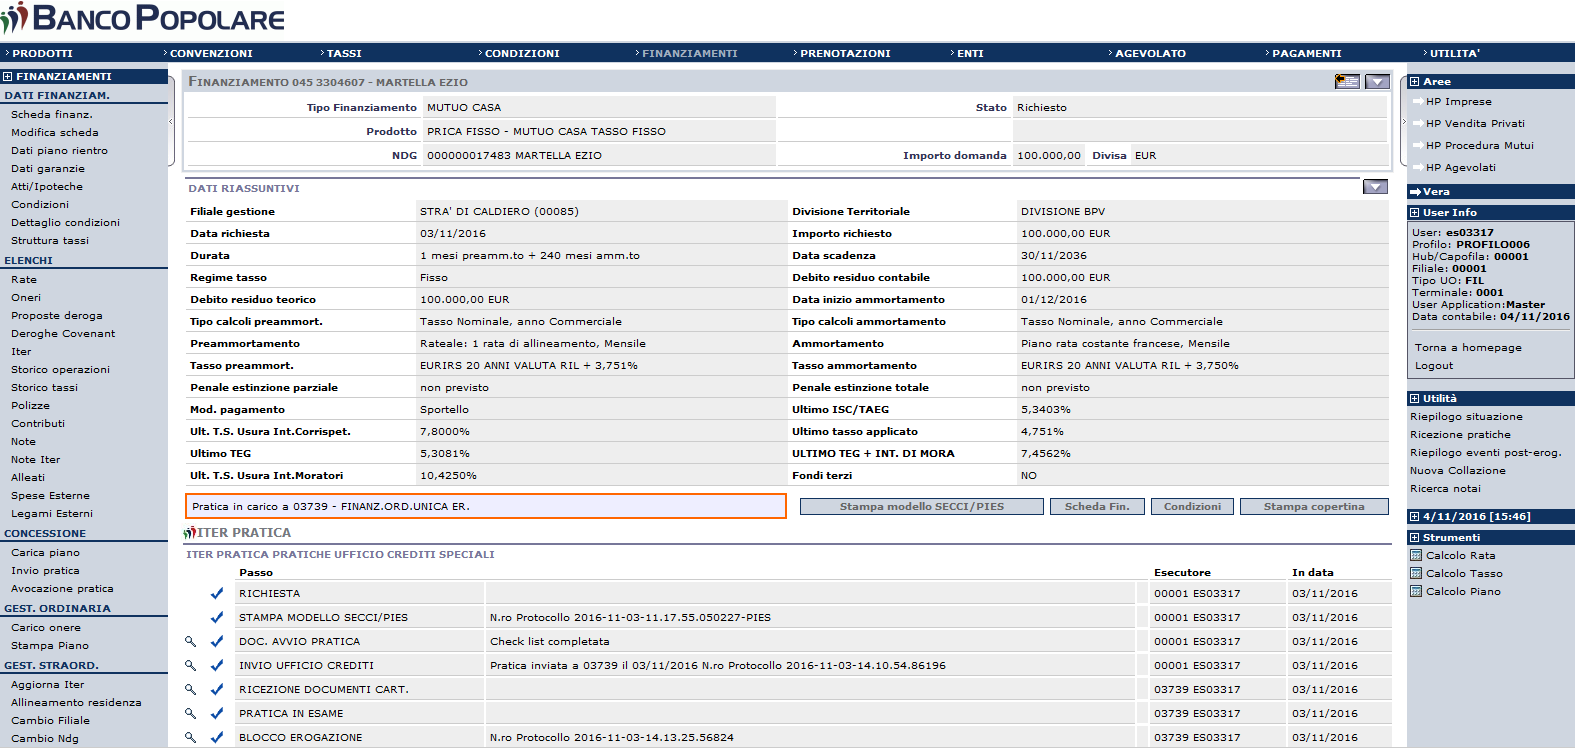
\includegraphics[width=1\textwidth]{immagini/interfaccia_ELISE}
	   	\caption{Interfaccia dell'applicazione ELISE - Fonte: Ambiente di sviluppo dell'applicazione}
	\end{figure}
	
	Il portale viene utilizzato ogni giorno dai dipendenti di ogni filiale del gruppo bancario. Rappresenta quindi un mezzo di nota importanza per il cliente	e l'erogazione dei suoi servizi.
	
	\subsection{Finalità del progetto}
	
	L'azienda ha l'obiettivo di espandersi e aumentare il proprio organico anche attraverso l'attivazione di stage con l'ottica di una futura assunzione; per questo i tirocinanti vengono inseriti nei team di sviluppo dei progetti già presi in carico per conto dei clienti. Il mio caso non ha fatto eccezione. \\
	
	Nel momento del mio inserimento in azienda, il progetto prevedeva nuove funzionalità da sviluppare. Il tutor aziendale ha quindi ritenuto adeguata una selezione di tali attività per caratterizzare il lavoro di stage, in previsione del fatto egli sarebbe stato presente per guidarmi soprattutto nelle prime fasi e successivamente educarmi all'autonomia.
	
	\newpage
	
	Il tutor si impegna in tal senso sia argomentando e motivando le scelte implementative che lo stagista è tenuto a prendere, sia lasciando la libertà di studiare soluzioni e alternative ai problemi proposti.\\
	
	Le attività che mi sono state assegnate nell'ultima fase di stage, dopo la formazione teorica e pratica, sono:

	\begin{itemize}
		\item \textbf{Aggiornamento stampe preventivo}: prima dell'erogazione di un finanziamento, il cliente è tenuto a valutare le offerte dei prodotti calcolandone i preventivi. L'applicazione già si occupa di generare i PDF di tale documentazione, ma vi era il bisogno di adeguare tali stampe a nuovi parametri e valori assicurativi.
		\item \textbf{Visualizzazione scadenziario covenant\glossario}: i finanziamenti bancari possono comprendere dei valori di convenzione attribuiti ad un certo periodo di validità. Era esigenza della banca poter visualizzare in modo intuitivo, con un calendario, le scadenze previste nei vari giorni e poterle analizzare nel dettaglio.	
		\item \textbf{Composizione titolari di un finanziamento}: era richiesto di creare una nuova pagina di visualizzazione dei titolari dei finanziamenti con la possibilità di modificarne, oltre a determinate categorie fiscali, la percentuale di titolarità. Inoltre dovevano essere implementate le logiche secondo cui, dopo la modifica ed il salvataggio dati, sarebbe dovuta apparire la possibilità di stampare la documentazione di sollevamento delle responsabilità da far firmare ai titolari.
		\item \textbf{Revisione funzionalità di ricerca tassi}: quest'attività prevedeva di implementare un filtro sul periodo di validità del valore dei tassi, per ottimizzare le performance della pagina di ricerca e presentazione dei risultati.
		\item \textbf{Ristrutturazione layout di una procedura}: nella procedura di attivazione di un finanziamento, un particolare passo di avanzamento riguarda la chiamata di un web service esterno, incluso nella pagina dell'applicativo mediante un iframe\glossario . Era richiesto di strutturare la presentazione di tale finestra e in particolare di sviluppare delle funzioni JavaScript per renderla ridimensionabile e trascinabile all'interno della pagina.
	\end{itemize}
	
	In questo percorso di espansione del software, l'azienda dispone di una risorsa in più per attuare il proprio lavoro e il soddisfacimento delle richieste del cliente riguardo il prodotto. Il tirocinante ne sarebbe quindi risultato maturato e munito di nuove conoscenze e abilità a lui utili ad un futuro lavorativo.\\
	
	L'applicativo è stato provvisto quindi di numerose aggiunte e modifiche utili all'adeguamento a nuovi termini legali in vigore, al miglioramento delle performance e della stabilità operativa e ovviamente alla predisposizione di nuove funzioni che amplificano il raggio d'azione e l'utilità di utilizzo per conto degli utenti.
	
	\subsection{Vincoli di progetto}

	\subsubsection{Imposti dal cliente}	
	Per quanto riguarda ELISE, il cliente ha esposto diversi vincoli per lo sviluppo.\\
	
	Alcuni sono impliciti nell'utilizzo di tecnologie, in particolare per interfacciarsi all'ambiente di gestione dati. L'applicazione adotta alcune librerie basate sulla Reflection\glossario\ per la codifica e la decodifica dei flussi dati, per la generazione di JavaBeans\glossario\ appositi. Un ulteriore vincolo tecnologico è rappresentato dalla necessità di mantenere compatibile il software per i browser utilizzati nelle filiali bancarie.\\
	
	Altri sono specificati ad ogni nuova richiesta di espansione dell'applicazione. Possono riguardare aspetti grafici, come la posizione di determinati elementi, oppure aspetti tecnici, come la necessità di garantire determinate performance per alcune funzionalità.\\
	
	Per il progetto ELISE e in particolare nelle attività a me attribuite, i vincoli riguardavano implementazioni specifiche:
	\begin{itemize}
		\item La necessità di ridurre il carico della pagina di visualizzazione dei valori tassi, implementando un filtro sul periodo di validità;
		\item Per la gestione dei titolari di un finanziamento il vincolo era di generare i documenti di stampa seguendo gli standard dell'applicazione;
		\item Per il layout dell'iframe\glossario , utile alla visualizzazione del servizio esterno, era richiesta la compatibilità con Microsoft Edge per garantire le prestazioni;
		\item Per lo scadenziario dei valori covenant\glossario , i vincoli riguardavano solo l'aspetto che doveva avere la pagina del calendario, per questo ho avuto una buona libertà di sviluppo.
	\end{itemize}

	\subsubsection{Imposti dall'azienda}	
	Dal punto di vista dell'azienda, l'obiettivo è sempre quello di innovare e apportare trasformazioni mirate all'adeguamento delle tecnologie utilizzate. Per questo motivo, a livello di sviluppo delle nuove funzionalità, vengono applicate sempre le ultime versioni delle tecnologie possibili, cercando di contrastare l'arretratezza dei meccanismi di programmazione web in ambito bancario.\\
	
	Sopra Steria però deve adottare anche le giuste precauzioni per far fronte alle spese dei progetti, per questo alle volte non è stato possibile impiegare troppo tempo per l'implementazione dei requisiti e di conseguenza pensare all'impiego di tecnologie più moderne.\\
	
	Anche tra i vincoli imposti dall'azienda, per il mio progetto di stage, vi sono stati diverse implicazioni tecnologiche.\\
	
	L'intera applicazione infatti si basa sull'architettura Java EE e il sistema di versionamento usato per coordinare i team di sviluppo e integrare il loro lavoro, è RTC. Di conseguenza ho dovuto studiare, imparare e mettere in pratica le tecnologie previste da tale architettura, come i JavaBeans\glossario\, le classi Servlet\glossario , le pagine JSP, i tag JSTL oltre ai linguaggi standard per la programmazione web HTML, CSS e JavaScript.

%**************************************************************
\section{Il mio stage in Sopra Steria}

Grazie alle offerte presenti a STAGE-IT 2016 e a molte altre che ho ricevuto, ho potuto selezionare le realtà lavorative che erano più orientate verso i miei criteri e ho deciso di partecipare al colloquio collettivo con Sopra Steria.\\

In particolare erano presenti circa 20 ragazzi che come me erano in procinto di laurearsi e volevano assicurarsi un posto in questa azienda. I recruiter hanno valutato il mio interesse e il potenziale che rappresentavo per loro nell'ambito sviluppativo in generale e il feedback è risultato positivo. Contando che per la sede di Padova erano a disposizione solamente due posti per attivare un tirocinio, mi sono sentito premiato e soddisfatto della mia scelta.\\

Il mio stage in Sopra Steria consisteva nello sviluppo di nuove funzioni per un applicativo web già operativo presso il cliente. Ho sviluppato tali funzionalità modificando e aggiungendo codice sorgente utilizzando Java EE e le tecnologie che mette a disposizione. Mi sono servito anche di Eclipse per agevolarmi nella realizzazione del progetto.

	\subsection{Motivo della scelta}
	
	Da quando mi sono avvicinato al mondo dell'informatica ho avuto il desiderio di toccare con mano situazioni di implementazione reale delle tecnologie che ho studiato, in particolare nell'ultimo anno dove ho avuto modo di trattare linguaggi e metodologie di programmazione moderni.\\
	
	Mi interessava quindi fare esperienza in ambito lavorativo e volevo distaccarmi da piccole realtà di sviluppo, per questo quando ho partecipato a diversi colloqui con aziende che cercavano stagisti per i loro progetti, ho avuto un occhio di riguardo all'ambiente in cui avrei lavorato.\\
	
	Ho tenuto conto inoltre del fatto che probabilmente in un secondo momento avrei potuto iniziare la mia carriera in tale contesto, come reso noto dalla maggioranza delle aziende che al giorno d'oggi cercano di ampliare il loro organico nel settore informatico. Questo è stato un ulteriore motivo che mi ha fatto cercare un'azienda di rilievo.\\
	
	Dei vari progetti che mi sono stati presentati, molti trattavano tecnologie certamente più innovative, ma Sopra Steria è stata comunque più convincente	sotto il punto di vista a lungo termine, offrendomi la possibilità in futuro di cambiare settore e ambito lavorativo in base alle mie esigenze e preferenze.
	
	\subsection{Obiettivi pianificati}
	
	All'interno del piano di lavoro del tirocinio io e il tutor aziendale abbiamo stabilito degli obiettivi da soddisfare per valutare positivamente l'attività di stage. La maggior parte riguardano lo svolgimento dello stage in azienda, altri invece sono relativi allo sviluppo dei progetti da me svolti. \\
	
	 I requisiti sono stati suddivisi in \textbf{obbligatori}: vincolanti in quanto primari e di diretto impatto sulla valutazione dello stage; \textbf{desiderabili}: non vincolanti o strettamente necessari, ma dal riconoscibile valore aggiuntivo; \textbf{facoltativi}: rappresentanti valore aggiuntivo non strettamente necessario.
	
	\subsubsection{Obbligatori}	
		\begin{itemize}
			\item Studio e acquisizione di padronanza dell'ambiente di sviluppo Eclipse;
			\item Studio e comprensione della piattaforma Java EE;
			\item Installazione e utilizzo di diversi \textit{application server} e diverse JVM;
			\item Acquisizione familiarità con la programmazione web in ambito Java (tecnologie JSP, JSTL, Servlet\glossario );
			\item Acquisizione tecniche di programmazione con framework Struts;
			\item Studio e utilizzo del sistema di versionamento RTC;
			\item Studio e utilizzo della tecnologia AJAX\glossario ;
			\item Implementazione di applicazioni di esempio per le funzionalità basilari;
			\item Analisi di una complessa applicazione reale in architettura Java EE;
			\item Integrazione nel team di sviluppo e acquisizione competenze nelle dinamiche di gruppo;
			\item Comprensione e acquisizione familiarità con la documentazione di analisi e specifica delle attività;
			\item Implementazione di modifiche basilari dell'applicazione ambito di progetto;
			\item Implementazione di modifiche complesse dell'applicazione ambito di progetto.
		\end{itemize}
		
	\subsubsection{Desiderabili}		
		\begin{itemize}
			\item Raggiungimento di un buon livello di autonomia nell'utilizzo di Java EE;
			\item Raggiungimento di un buon livello di autonomia nell'utilizzo di tecnologie web standard (HTML, CSS, JavaScript);
			\item Raggiungimento di un buon livello di autonomia nell'utilizzo di tecnologie web in ambito Java (JSP, JSTL, Servlet\glossario );
			\item Acquisizione tecniche di programmazione con framework alternativi (Maven e Hibernate);
			\item Studio e utilizzo di un sistema di versionamento alternativo (SVN);
			\item Studio e utilizzo della libreria per le stampe PDF, iText;
			\item Studio e utilizzo della libreria per il \textit{logging}, Log4J;
			\item Capacità di portare a termine le attività lavorative secondo le tempistiche stabilite, anche in situazioni critiche;
			\item Conoscenza delle norme di sicurezza relative all'ambiente di lavoro.
		\end{itemize}
		
	\subsubsection{Facoltativi}	
		\begin{itemize}
			\item Studio delle meccaniche di comunicazione con l'area di business per la gestione dei dati;
			\item Partecipazione alle attività di test di integrazione dell'applicazione ambito di progetto;
			\item Partecipazione alle attività di collaudo dell'applicazione ambito di progetto;
			\item Rilascio delle nuove funzionalità sviluppate nelle attività assegnate.
		\end{itemize}
		
	Il grafico in figura \ref{suddivisione-obiettivi} mostra la suddivisione degli obiettivi nelle diverse tipologie, facendo notare che quelli obbligatori compongono il 50\% dei totali concordati e l'altra	metà si suddivide in desiderabili e facoltativi.\\
	
	\begin{figure}[H]
		\centering
	   	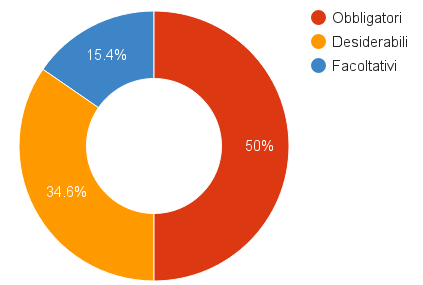
\includegraphics[width=0.7\textwidth]{immagini/suddivisione_obiettivi}
	   	\caption{Suddivisione degli obiettivi dello stage}
	   	\vspace{2mm}
	   	\label{suddivisione-obiettivi}
	\end{figure}

	\subsection{Obiettivi personali}
	
	Iniziando lo stage, le mie aspettative erano piuttosto semplici: desideravo apprendere nuove tecnologie per la programmazione web, in modo da ampliare le mie conoscenze a riguardo e specializzarmi abbastanza in questo ambito per giocare un ruolo chiave nelle attività dell'azienda.\\
	
	Mi aspettavo di lavorare inizialmente in un ambiente distaccato dai team di sviluppo per un periodo iniziale, in modo da formarmi adeguatamente e poi entrare in contatto con il mondo lavorativo vero e proprio per dare il mio contributo.\\
	
	Volevo ampliare profondamente le mie conoscenze riguardo gli ambienti di sviluppo che sarei andato ad utilizzare e le tecniche previste nell'ambito in cui sarei stato inserito: creazione di progetti, inserimento e sviluppo di nuove parti nei prodotti e utilizzo di debugging.\\
	
	Speravo di andare a conoscere i più diffusi framework e le più diffuse librerie	presenti, imparando a utilizzarli al meglio. Il linguaggio Java, impiegato in modo massiccio per questo stage, era già di mia conoscenza grazie al percorso di studi offerto dall'Università, ma la sua applicazione in ambito web mi era ancora sconosciuta e volevo comprendere al meglio i meccanismi e le tecnologie che permettono tale tipo di sviluppi.\\
	
	Gli altri linguaggi per la realizzazione di pagine web erano già di mia conoscenza, desideravo applicarli in un progetto realmente utilizzato e guadagnare autonomia nella loro applicazione per completare il percorso di apprendimento.\\
	
	Desideravo formarmi professionalmente, accrescere il mio potenziale in ambito lavorativo e al contempo diventare autonomo nelle mie attività; senza	sottovalutare però l'interesse verso i casi implementativi, perché volevo trasformare quello che speravo diventasse il mio futuro lavoro in una passione.